% Created by tikzDevice version 0.10.1 on 2018-06-21 09:33:53
% !TEX encoding = UTF-8 Unicode
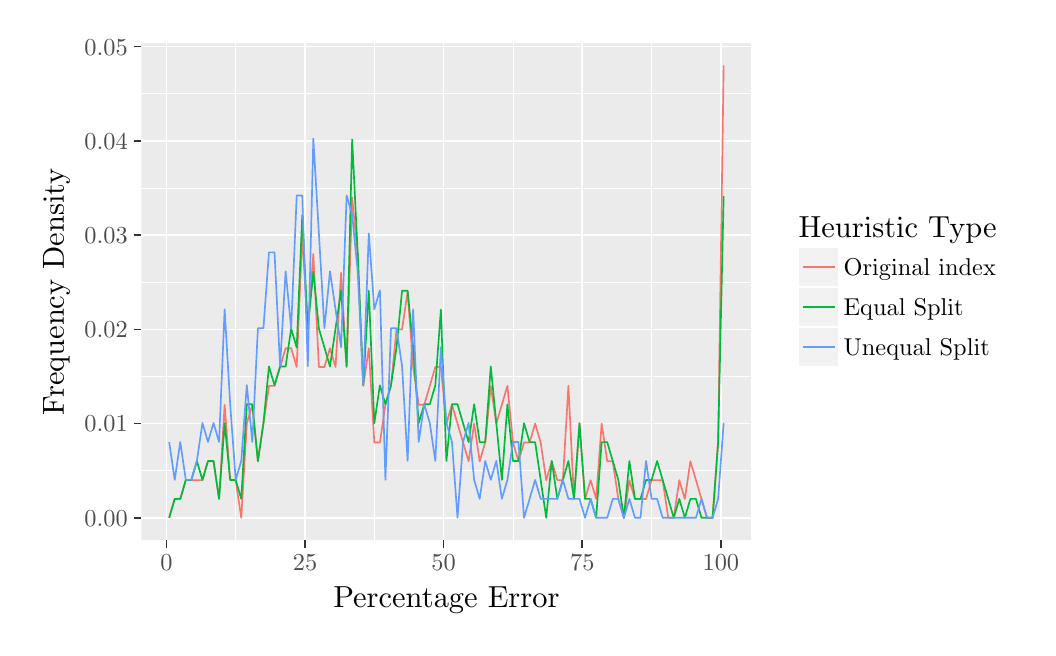
\begin{tikzpicture}[x=1pt,y=1pt]
\definecolor{fillColor}{RGB}{255,255,255}
\path[use as bounding box,fill=fillColor,fill opacity=0.00] (0,0) rectangle (361.35,216.81);
\begin{scope}
\path[clip] (  0.00,  0.00) rectangle (361.35,216.81);
\definecolor{drawColor}{RGB}{255,255,255}
\definecolor{fillColor}{RGB}{255,255,255}

\path[draw=drawColor,line width= 0.6pt,line join=round,line cap=round,fill=fillColor] (  0.00,  0.00) rectangle (361.35,216.81);
\end{scope}
\begin{scope}
\path[clip] ( 41.11, 31.53) rectangle (261.51,211.31);
\definecolor{fillColor}{gray}{0.92}

\path[fill=fillColor] ( 41.11, 31.53) rectangle (261.51,211.31);
\definecolor{drawColor}{RGB}{255,255,255}

\path[draw=drawColor,line width= 0.3pt,line join=round] ( 41.11, 56.73) --
	(261.51, 56.73);

\path[draw=drawColor,line width= 0.3pt,line join=round] ( 41.11, 90.78) --
	(261.51, 90.78);

\path[draw=drawColor,line width= 0.3pt,line join=round] ( 41.11,124.83) --
	(261.51,124.83);

\path[draw=drawColor,line width= 0.3pt,line join=round] ( 41.11,158.87) --
	(261.51,158.87);

\path[draw=drawColor,line width= 0.3pt,line join=round] ( 41.11,192.92) --
	(261.51,192.92);

\path[draw=drawColor,line width= 0.3pt,line join=round] ( 75.17, 31.53) --
	( 75.17,211.31);

\path[draw=drawColor,line width= 0.3pt,line join=round] (125.26, 31.53) --
	(125.26,211.31);

\path[draw=drawColor,line width= 0.3pt,line join=round] (175.36, 31.53) --
	(175.36,211.31);

\path[draw=drawColor,line width= 0.3pt,line join=round] (225.45, 31.53) --
	(225.45,211.31);

\path[draw=drawColor,line width= 0.6pt,line join=round] ( 41.11, 39.70) --
	(261.51, 39.70);

\path[draw=drawColor,line width= 0.6pt,line join=round] ( 41.11, 73.75) --
	(261.51, 73.75);

\path[draw=drawColor,line width= 0.6pt,line join=round] ( 41.11,107.80) --
	(261.51,107.80);

\path[draw=drawColor,line width= 0.6pt,line join=round] ( 41.11,141.85) --
	(261.51,141.85);

\path[draw=drawColor,line width= 0.6pt,line join=round] ( 41.11,175.90) --
	(261.51,175.90);

\path[draw=drawColor,line width= 0.6pt,line join=round] ( 41.11,209.95) --
	(261.51,209.95);

\path[draw=drawColor,line width= 0.6pt,line join=round] ( 50.13, 31.53) --
	( 50.13,211.31);

\path[draw=drawColor,line width= 0.6pt,line join=round] (100.22, 31.53) --
	(100.22,211.31);

\path[draw=drawColor,line width= 0.6pt,line join=round] (150.31, 31.53) --
	(150.31,211.31);

\path[draw=drawColor,line width= 0.6pt,line join=round] (200.40, 31.53) --
	(200.40,211.31);

\path[draw=drawColor,line width= 0.6pt,line join=round] (250.49, 31.53) --
	(250.49,211.31);
\definecolor{drawColor}{RGB}{248,118,109}

\path[draw=drawColor,line width= 0.6pt,line join=round] ( 51.13, 39.70) --
	( 53.13, 46.51) --
	( 55.14, 46.51) --
	( 57.14, 53.32) --
	( 59.14, 53.32) --
	( 61.15, 53.32) --
	( 63.15, 53.32) --
	( 65.15, 60.13) --
	( 67.16, 60.13) --
	( 69.16, 46.51) --
	( 71.17, 80.56) --
	( 73.17, 53.32) --
	( 75.17, 53.32) --
	( 77.18, 39.70) --
	( 79.18, 73.75) --
	( 81.18, 80.56) --
	( 83.19, 60.13) --
	( 85.19, 73.75) --
	( 87.19, 87.37) --
	( 89.20, 87.37) --
	( 91.20, 94.18) --
	( 93.21,100.99) --
	( 95.21,100.99) --
	( 97.21, 94.18) --
	( 99.22,141.85) --
	(101.22,107.80) --
	(103.22,135.04) --
	(105.23, 94.18) --
	(107.23, 94.18) --
	(109.24,100.99) --
	(111.24, 94.18) --
	(113.24,128.23) --
	(115.25, 94.18) --
	(117.25,155.47) --
	(119.25,135.04) --
	(121.26, 87.37) --
	(123.26,100.99) --
	(125.26, 66.94) --
	(127.27, 66.94) --
	(129.27, 80.56) --
	(131.28, 87.37) --
	(133.28,107.80) --
	(135.28,107.80) --
	(137.29,121.42) --
	(139.29, 94.18) --
	(141.29, 80.56) --
	(143.30, 80.56) --
	(145.30, 87.37) --
	(147.30, 94.18) --
	(149.31, 94.18) --
	(151.31, 73.75) --
	(153.32, 80.56) --
	(155.32, 73.75) --
	(157.32, 66.94) --
	(159.33, 60.13) --
	(161.33, 73.75) --
	(163.33, 60.13) --
	(165.34, 66.94) --
	(167.34, 87.37) --
	(169.34, 73.75) --
	(171.35, 80.56) --
	(173.35, 87.37) --
	(175.36, 66.94) --
	(177.36, 60.13) --
	(179.36, 66.94) --
	(181.37, 66.94) --
	(183.37, 73.75) --
	(185.37, 66.94) --
	(187.38, 53.32) --
	(189.38, 60.13) --
	(191.39, 53.32) --
	(193.39, 53.32) --
	(195.39, 87.37) --
	(197.40, 46.51) --
	(199.40, 73.75) --
	(201.40, 46.51) --
	(203.41, 53.32) --
	(205.41, 46.51) --
	(207.41, 73.75) --
	(209.42, 60.13) --
	(211.42, 60.13) --
	(213.43, 46.51) --
	(215.43, 39.70) --
	(217.43, 53.32) --
	(219.44, 46.51) --
	(221.44, 46.51) --
	(223.44, 46.51) --
	(225.45, 53.32) --
	(227.45, 53.32) --
	(229.45, 53.32) --
	(231.46, 39.70) --
	(233.46, 39.70) --
	(235.47, 53.32) --
	(237.47, 46.51) --
	(239.47, 60.13) --
	(241.48, 53.32) --
	(243.48, 46.51) --
	(245.48, 39.70) --
	(247.49, 39.70) --
	(249.49, 66.94) --
	(251.49,203.14);
\definecolor{drawColor}{RGB}{0,186,56}

\path[draw=drawColor,line width= 0.6pt,line join=round] ( 51.13, 39.70) --
	( 53.13, 46.54) --
	( 55.14, 46.54) --
	( 57.14, 53.38) --
	( 59.14, 53.38) --
	( 61.15, 60.21) --
	( 63.15, 53.38) --
	( 65.15, 60.21) --
	( 67.16, 60.21) --
	( 69.16, 46.54) --
	( 71.17, 73.89) --
	( 73.17, 53.38) --
	( 75.17, 53.38) --
	( 77.18, 46.54) --
	( 79.18, 80.73) --
	( 81.18, 80.73) --
	( 83.19, 60.21) --
	( 85.19, 73.89) --
	( 87.19, 94.40) --
	( 89.20, 87.56) --
	( 91.20, 94.40) --
	( 93.21, 94.40) --
	( 95.21,108.07) --
	( 97.21,101.24) --
	( 99.22,149.10) --
	(101.22,108.07) --
	(103.22,128.59) --
	(105.23,108.07) --
	(107.23,101.24) --
	(109.24, 94.40) --
	(111.24,108.07) --
	(113.24,121.75) --
	(115.25, 94.40) --
	(117.25,176.45) --
	(119.25,135.42) --
	(121.26, 87.56) --
	(123.26,121.75) --
	(125.26, 73.89) --
	(127.27, 87.56) --
	(129.27, 80.73) --
	(131.28, 87.56) --
	(133.28,101.24) --
	(135.28,121.75) --
	(137.29,121.75) --
	(139.29,101.24) --
	(141.29, 73.89) --
	(143.30, 80.73) --
	(145.30, 80.73) --
	(147.30, 87.56) --
	(149.31,114.91) --
	(151.31, 60.21) --
	(153.32, 80.73) --
	(155.32, 80.73) --
	(157.32, 73.89) --
	(159.33, 67.05) --
	(161.33, 80.73) --
	(163.33, 67.05) --
	(165.34, 67.05) --
	(167.34, 94.40) --
	(169.34, 73.89) --
	(171.35, 53.38) --
	(173.35, 80.73) --
	(175.36, 60.21) --
	(177.36, 60.21) --
	(179.36, 73.89) --
	(181.37, 67.05) --
	(183.37, 67.05) --
	(185.37, 53.38) --
	(187.38, 39.70) --
	(189.38, 60.21) --
	(191.39, 46.54) --
	(193.39, 53.38) --
	(195.39, 60.21) --
	(197.40, 46.54) --
	(199.40, 73.89) --
	(201.40, 46.54) --
	(203.41, 46.54) --
	(205.41, 39.70) --
	(207.41, 67.05) --
	(209.42, 67.05) --
	(211.42, 60.21) --
	(213.43, 53.38) --
	(215.43, 39.70) --
	(217.43, 60.21) --
	(219.44, 46.54) --
	(221.44, 46.54) --
	(223.44, 53.38) --
	(225.45, 53.38) --
	(227.45, 60.21) --
	(229.45, 53.38) --
	(231.46, 46.54) --
	(233.46, 39.70) --
	(235.47, 46.54) --
	(237.47, 39.70) --
	(239.47, 46.54) --
	(241.48, 46.54) --
	(243.48, 39.70) --
	(245.48, 39.70) --
	(247.49, 39.70) --
	(249.49, 67.05) --
	(251.49,155.93);
\definecolor{drawColor}{RGB}{97,156,255}

\path[draw=drawColor,line width= 0.6pt,line join=round] ( 51.13, 67.11) --
	( 53.13, 53.40) --
	( 55.14, 67.11) --
	( 57.14, 53.40) --
	( 59.14, 53.40) --
	( 61.15, 60.26) --
	( 63.15, 73.96) --
	( 65.15, 67.11) --
	( 67.16, 73.96) --
	( 69.16, 67.11) --
	( 71.17,115.06) --
	( 73.17, 80.81) --
	( 75.17, 53.40) --
	( 77.18, 60.26) --
	( 79.18, 87.66) --
	( 81.18, 67.11) --
	( 83.19,108.21) --
	( 85.19,108.21) --
	( 87.19,135.62) --
	( 89.20,135.62) --
	( 91.20, 94.51) --
	( 93.21,128.76) --
	( 95.21,108.21) --
	( 97.21,156.17) --
	( 99.22,156.17) --
	(101.22, 94.51) --
	(103.22,176.72) --
	(105.23,142.47) --
	(107.23,108.21) --
	(109.24,128.76) --
	(111.24,115.06) --
	(113.24,101.36) --
	(115.25,156.17) --
	(117.25,149.32) --
	(119.25,128.76) --
	(121.26, 87.66) --
	(123.26,142.47) --
	(125.26,115.06) --
	(127.27,121.91) --
	(129.27, 53.40) --
	(131.28,108.21) --
	(133.28,108.21) --
	(135.28, 94.51) --
	(137.29, 60.26) --
	(139.29,115.06) --
	(141.29, 67.11) --
	(143.30, 80.81) --
	(145.30, 73.96) --
	(147.30, 60.26) --
	(149.31,101.36) --
	(151.31, 73.96) --
	(153.32, 67.11) --
	(155.32, 39.70) --
	(157.32, 67.11) --
	(159.33, 73.96) --
	(161.33, 53.40) --
	(163.33, 46.55) --
	(165.34, 60.26) --
	(167.34, 53.40) --
	(169.34, 60.26) --
	(171.35, 46.55) --
	(173.35, 53.40) --
	(175.36, 67.11) --
	(177.36, 67.11) --
	(179.36, 39.70) --
	(181.37, 46.55) --
	(183.37, 53.40) --
	(185.37, 46.55) --
	(187.38, 46.55) --
	(189.38, 46.55) --
	(191.39, 46.55) --
	(193.39, 53.40) --
	(195.39, 46.55) --
	(197.40, 46.55) --
	(199.40, 46.55) --
	(201.40, 39.70) --
	(203.41, 46.55) --
	(205.41, 39.70) --
	(207.41, 39.70) --
	(209.42, 39.70) --
	(211.42, 46.55) --
	(213.43, 46.55) --
	(215.43, 39.70) --
	(217.43, 46.55) --
	(219.44, 39.70) --
	(221.44, 39.70) --
	(223.44, 60.26) --
	(225.45, 46.55) --
	(227.45, 46.55) --
	(229.45, 39.70) --
	(231.46, 39.70) --
	(233.46, 39.70) --
	(235.47, 39.70) --
	(237.47, 39.70) --
	(239.47, 39.70) --
	(241.48, 39.70) --
	(243.48, 46.55) --
	(245.48, 39.70) --
	(247.49, 39.70) --
	(249.49, 46.55) --
	(251.49, 73.96);
\end{scope}
\begin{scope}
\path[clip] (  0.00,  0.00) rectangle (361.35,216.81);
\definecolor{drawColor}{gray}{0.30}

\node[text=drawColor,anchor=base east,inner sep=0pt, outer sep=0pt, scale=  0.88] at ( 36.16, 36.67) {0.00};

\node[text=drawColor,anchor=base east,inner sep=0pt, outer sep=0pt, scale=  0.88] at ( 36.16, 70.72) {0.01};

\node[text=drawColor,anchor=base east,inner sep=0pt, outer sep=0pt, scale=  0.88] at ( 36.16,104.77) {0.02};

\node[text=drawColor,anchor=base east,inner sep=0pt, outer sep=0pt, scale=  0.88] at ( 36.16,138.82) {0.03};

\node[text=drawColor,anchor=base east,inner sep=0pt, outer sep=0pt, scale=  0.88] at ( 36.16,172.87) {0.04};

\node[text=drawColor,anchor=base east,inner sep=0pt, outer sep=0pt, scale=  0.88] at ( 36.16,206.92) {0.05};
\end{scope}
\begin{scope}
\path[clip] (  0.00,  0.00) rectangle (361.35,216.81);
\definecolor{drawColor}{gray}{0.20}

\path[draw=drawColor,line width= 0.6pt,line join=round] ( 38.36, 39.70) --
	( 41.11, 39.70);

\path[draw=drawColor,line width= 0.6pt,line join=round] ( 38.36, 73.75) --
	( 41.11, 73.75);

\path[draw=drawColor,line width= 0.6pt,line join=round] ( 38.36,107.80) --
	( 41.11,107.80);

\path[draw=drawColor,line width= 0.6pt,line join=round] ( 38.36,141.85) --
	( 41.11,141.85);

\path[draw=drawColor,line width= 0.6pt,line join=round] ( 38.36,175.90) --
	( 41.11,175.90);

\path[draw=drawColor,line width= 0.6pt,line join=round] ( 38.36,209.95) --
	( 41.11,209.95);
\end{scope}
\begin{scope}
\path[clip] (  0.00,  0.00) rectangle (361.35,216.81);
\definecolor{drawColor}{gray}{0.20}

\path[draw=drawColor,line width= 0.6pt,line join=round] ( 50.13, 28.78) --
	( 50.13, 31.53);

\path[draw=drawColor,line width= 0.6pt,line join=round] (100.22, 28.78) --
	(100.22, 31.53);

\path[draw=drawColor,line width= 0.6pt,line join=round] (150.31, 28.78) --
	(150.31, 31.53);

\path[draw=drawColor,line width= 0.6pt,line join=round] (200.40, 28.78) --
	(200.40, 31.53);

\path[draw=drawColor,line width= 0.6pt,line join=round] (250.49, 28.78) --
	(250.49, 31.53);
\end{scope}
\begin{scope}
\path[clip] (  0.00,  0.00) rectangle (361.35,216.81);
\definecolor{drawColor}{gray}{0.30}

\node[text=drawColor,anchor=base,inner sep=0pt, outer sep=0pt, scale=  0.88] at ( 50.13, 20.52) {0};

\node[text=drawColor,anchor=base,inner sep=0pt, outer sep=0pt, scale=  0.88] at (100.22, 20.52) {25};

\node[text=drawColor,anchor=base,inner sep=0pt, outer sep=0pt, scale=  0.88] at (150.31, 20.52) {50};

\node[text=drawColor,anchor=base,inner sep=0pt, outer sep=0pt, scale=  0.88] at (200.40, 20.52) {75};

\node[text=drawColor,anchor=base,inner sep=0pt, outer sep=0pt, scale=  0.88] at (250.49, 20.52) {100};
\end{scope}
\begin{scope}
\path[clip] (  0.00,  0.00) rectangle (361.35,216.81);
\definecolor{drawColor}{RGB}{0,0,0}

\node[text=drawColor,anchor=base,inner sep=0pt, outer sep=0pt, scale=  1.10] at (151.31,  7.44) {Percentage Error};
\end{scope}
\begin{scope}
\path[clip] (  0.00,  0.00) rectangle (361.35,216.81);
\definecolor{drawColor}{RGB}{0,0,0}

\node[text=drawColor,rotate= 90.00,anchor=base,inner sep=0pt, outer sep=0pt, scale=  1.10] at ( 13.08,121.42) {Frequency Density};
\end{scope}
\begin{scope}
\path[clip] (  0.00,  0.00) rectangle (361.35,216.81);
\definecolor{fillColor}{RGB}{255,255,255}

\path[fill=fillColor] (272.89, 88.45) rectangle (355.85,154.39);
\end{scope}
\begin{scope}
\path[clip] (  0.00,  0.00) rectangle (361.35,216.81);
\definecolor{drawColor}{RGB}{0,0,0}

\node[text=drawColor,anchor=base west,inner sep=0pt, outer sep=0pt, scale=  1.10] at (278.58,141.12) {Heuristic Type};
\end{scope}
\begin{scope}
\path[clip] (  0.00,  0.00) rectangle (361.35,216.81);
\definecolor{drawColor}{RGB}{255,255,255}
\definecolor{fillColor}{gray}{0.95}

\path[draw=drawColor,line width= 0.6pt,line join=round,line cap=round,fill=fillColor] (278.58,123.05) rectangle (293.04,137.51);
\end{scope}
\begin{scope}
\path[clip] (  0.00,  0.00) rectangle (361.35,216.81);
\definecolor{drawColor}{RGB}{248,118,109}

\path[draw=drawColor,line width= 0.6pt,line join=round] (280.03,130.28) -- (291.59,130.28);
\end{scope}
\begin{scope}
\path[clip] (  0.00,  0.00) rectangle (361.35,216.81);
\definecolor{drawColor}{RGB}{255,255,255}
\definecolor{fillColor}{gray}{0.95}

\path[draw=drawColor,line width= 0.6pt,line join=round,line cap=round,fill=fillColor] (278.58,108.60) rectangle (293.04,123.05);
\end{scope}
\begin{scope}
\path[clip] (  0.00,  0.00) rectangle (361.35,216.81);
\definecolor{drawColor}{RGB}{0,186,56}

\path[draw=drawColor,line width= 0.6pt,line join=round] (280.03,115.83) -- (291.59,115.83);
\end{scope}
\begin{scope}
\path[clip] (  0.00,  0.00) rectangle (361.35,216.81);
\definecolor{drawColor}{RGB}{255,255,255}
\definecolor{fillColor}{gray}{0.95}

\path[draw=drawColor,line width= 0.6pt,line join=round,line cap=round,fill=fillColor] (278.58, 94.14) rectangle (293.04,108.60);
\end{scope}
\begin{scope}
\path[clip] (  0.00,  0.00) rectangle (361.35,216.81);
\definecolor{drawColor}{RGB}{97,156,255}

\path[draw=drawColor,line width= 0.6pt,line join=round] (280.03,101.37) -- (291.59,101.37);
\end{scope}
\begin{scope}
\path[clip] (  0.00,  0.00) rectangle (361.35,216.81);
\definecolor{drawColor}{RGB}{0,0,0}

\node[text=drawColor,anchor=base west,inner sep=0pt, outer sep=0pt, scale=  0.88] at (294.85,127.25) {Original index};
\end{scope}
\begin{scope}
\path[clip] (  0.00,  0.00) rectangle (361.35,216.81);
\definecolor{drawColor}{RGB}{0,0,0}

\node[text=drawColor,anchor=base west,inner sep=0pt, outer sep=0pt, scale=  0.88] at (294.85,112.80) {Equal Split};
\end{scope}
\begin{scope}
\path[clip] (  0.00,  0.00) rectangle (361.35,216.81);
\definecolor{drawColor}{RGB}{0,0,0}

\node[text=drawColor,anchor=base west,inner sep=0pt, outer sep=0pt, scale=  0.88] at (294.85, 98.34) {Unequal Split};
\end{scope}
\end{tikzpicture}
